\documentclass[a4paper,11pt,notitlepage]{article}
\usepackage[utf8]{inputenc}	% latin2 - kodowanie iso-8859-2; cp1250 - kodowanie windows
\usepackage[T1]{fontenc}
\usepackage{enumitem}
\usepackage[polish]{babel}
\usepackage[MeX]{polski}
\usepackage{graphicx}
\selectlanguage{polish}

\usepackage{graphicx}

\hyphenation{FreeBSD}

\author{Wojciech Świstowski (252572)}
\title{Specyfikacja Implementacyjna projektu Problem N-Ciał}
\date{\today}

\linespread{1.3}

\usepackage{indentfirst}

\begin{document}
\maketitle

\section{Podział programu na moduły}

Program zostanie podzielony na 5 modułów, według poniższego schematu:
\begin{figure}[ht!]
\centering
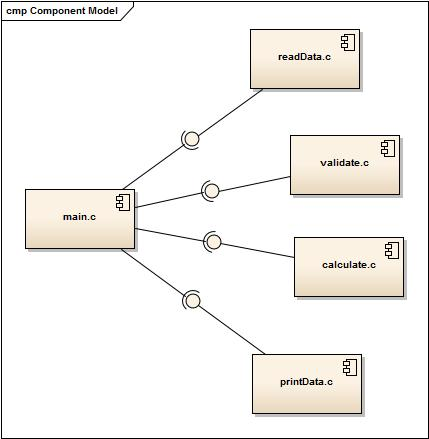
\includegraphics[width=0.75\textwidth]{moduly.jpg}
\end{figure}

\section{Funkcje programu}
Implementacja projektu będzie zawierać 10 głównych funkcji, które  dla przejrzystości kodu rozdzielone zostaną pomiędzy modułami według podobieństw funkcjonalności. Przyporządkowanie funkcji do modułów odbędzie się w poniższy sposób:
\begin{enumerate}[noitemsep]
	\item readData.c
	\begin{itemize}
		\item Wczytywanie danych z plików wejściowych:
		\footnotesize\begin{verbatim}
		struct body *readData(char **filename, int nFiles)
		\end{verbatim}\normalsize
		\item Zliczanie ciał:
		\footnotesize\begin{verbatim}
		int checkBodyAmount(char **filename, int nFiles)
		\end{verbatim}\normalsize
	\end{itemize}
	\item printData.c
	\begin{itemize}
		\item Zapisywanie iteracji do plików wyjściowych:
		\footnotesize\begin{verbatim}
		void printIterationToFile(char **fileNames, int size)
		\end{verbatim}\normalsize
		\item Wypisywanie wczytanych danych na ekran:
		\footnotesize\begin{verbatim}
		void printData(struct body *dataBank, int size)
		\end{verbatim}\normalsize
	\end{itemize}
	\item calculate.c
	\begin{itemize}
		\item Obliczanie nowej pozycji ciała:
		\footnotesize\begin{verbatim}
		void calculateNewPosition(int index, long timeDiff, int size)
		\end{verbatim}\normalsize
		\item Przeliczanie na sekundy czasu z parametrów wejściowych programu:
		\footnotesize\begin{verbatim}
		long calculateTime(long value, char unit)
		\end{verbatim}\normalsize
		\item Obliczanie pozycji wszystkich ciał we wszystkich iteracjach:
		\footnotesize\begin{verbatim}
		void calculateAllPositions(int size, long timeDiff)
		\end{verbatim}\normalsize
	\end{itemize}
	\item validate.c
	\begin{itemize}
		\item Sprawdzenie liczby plików wejściowych:
		\footnotesize\begin{verbatim}
		void checkFileNumber(int fileNumber, int numberOfArguments)
		\end{verbatim}\normalsize
		\item Sprawdzenie czy wprowadzony argument wejściowy jest liczbą:
		\footnotesize\begin{verbatim}
		void checkNumericArgument(char *argument)
		\end{verbatim}\normalsize
		\item Sprawdzenie kompletności danych:
		\footnotesize\begin{verbatim}
		void checkForMissingData ()
		\end{verbatim}\normalsize
	\end{itemize}
\end{enumerate}

\section{Opis struktur}
Do zaimplementowania programu użyta zostanie tylko jedna struktura danych:

		\footnotesize\begin{verbatim}
		struct body {
    		char *name;
   			double mass;
    		double posX;
    		double posY;
    		double posZ;
    		double velocityX;
    		double velocityY;
    		double velocityZ;
		}
		\end{verbatim}\normalsize
		
Struktura ta będzie przechowywała dane na temat ciał w obecnie obliczanej iteracji.

\section{Dodatkowe biblioteki}
Projekt będzie wykorzystywał poniższe biblioteki:
\begin{itemize}
		\item stdio.h
		\item stdlib.h
		\item string.h
		\item math.h
		\item sys/stat.h
	\end{itemize}

\section{Testowanie}

Podczas testowanie wykorzystywanych będzie przynajmniej kilka różnych plików wejściowych i wiele kombinacji argumentów wywołania programu. Sprawdzane będzie działanie programu dla: jednego, kilku plików wejściowych jak i braku takich plików (podane złe nazwy lub nie podano nazwy pliku wejściowego). Bardzo ważne będą testy dla przypadków, które mogą wywołać nieprawidłowe działanie programu. Szczególną uwagę należy zwrócić na poniższe scenariusze:
\begin{itemize}
 		\item dane wejściowe dublujące się
 		\item dane wejściowe niekompletne
 		\item pusty plik wejściowy
 		\item brak plików wejściowych
 		\item nieprawidłowe argumenty wywołania.
\end{itemize}
 \end{document}
